\chapter{Background}
\label{cha:background}
The Stratosphere is a layer of the Earth's atmosphere characterised by increasing temperatures with height. This feature distinguishes it from the lowest layer of the atmosphere, the troposphere, and makes it stable to vertical convection. As a result, the stratosphere exhibits significantly different dynamical behaviour to the troposphere. The stratosphere is bounded by the tropopause from below and the stratopause above. The height of these bounds vary latitudinally with tropopause heights ranging from  xxx at the equator to $\sim$ xxx km in the polar regions. While the stratosphere and troposphere are characterised seperately, current understanding of atmospheric dynamics incorporates elements of coupling between the layers. This chapter outlines the key points of this current understanding including dynamics of the polar and equatorial stratosphere, stratosphere-troposphere coupling as well as surface variability relevant to the stratosphere.


\section{The Stratospheric Polar Vortex}
\label{sec:polar_vortex}
During Northern Hemisphere (NH) winter, the NH polar stratosphere is plunged into polar night. As a result, it experiences a net cooling effect through emission of longwave infrared radiation to space and the absence of shortwave solar radiation available for absorption. This significant cooling increases the meridional temperature gradient between the polar region and the tropics. This causes an increase in the vertical shear of zonal wind according to the thermal wind balance relation,

\begin{equation} \label{eq:thermal_wind}
\frac{\partial u_g}{\partial z} = -\frac{R}{f H}\frac{\partial T}{\partial y},
\end{equation}

where $u_g$ is the geostrophic zonal wind velocity (the wind resulting in a balance between Coriolis and pressure gradient forces), $z$ is the height coordinate, $R$ is the specific gas constant and $H$ is the atmospheric scale height, the gain in altitude which leads to a reduction in atmospheric pressure by a factor of $e$ given by $H = RT_r/g$ (g = acceleration d due to gravity and $T_r$ is a reference temperature). $f$ in equation \ref{eq:thermal_wind} is the Coriolis parameter under a beta plane approximation which is given by

\begin{equation} \label{eq:beta_plane_approx}
f = f_0 + \beta y = 2 \Omega sin(\phi_0) + 2 \Omega cos(\phi_0)\frac{ y}{a},
\end{equation}

where $\phi_0$ is a reference latitude, $\Omega$ is the rotation rate of the earth and $a$ is the Earth's radius. This increase in vertical shear in $u_g$ leads to a strong, stratospheric, westerly flow circumnavigating the North Pole during boreal winter months. This feature is known as the northern hemisphere polar vortex or polar night jet. Henceforth we refer to it as the vortex.

The vortex contains a core of cold polar air in which temperatures can drop to around 200K in the lower stratosphere according to the European Centre for Medium Range Weather Forecasting (ECMWF) interim reanalysis data set (referred to as ERA-interim). Wintertime averaged zonal wind speeds are found to reach up to approximately $40ms^{-1}$ at the 10hPa level at a latitude of 60N. Figure \ref{fig:ERAclimDJF} shows the climatological zonal mean zonal wind (ZMZW) from ERA-interim for the December-February period. It exhibits the traits set out above with a persistent zonal westerly wind above the 30hPa level. The troposphere exhibits 2 westerly jets which show greatest magnitude winds at approximately xxx hPa. Also included in figure \ref{fig:ERAclimDJF} is the seasonal cycle in daily winds at 60N on the 10hPa level (near the edge of the vortex). On average, the vortex forms in mid xxxx and breaks down to be replaced with summer easterlies in xxx. These winds show a large degree of variability across different seasons (figure \ref{fig:ERAclimDJF} grey lines) with some seasons exhibiting anomalously strong westerly flow and others even exhibiting easterlies for a portion of the season. These effects are due to the action of atmospheric waves on the vortex and are described fully in the following section. 


\begin{figure}[h!]
\centering
    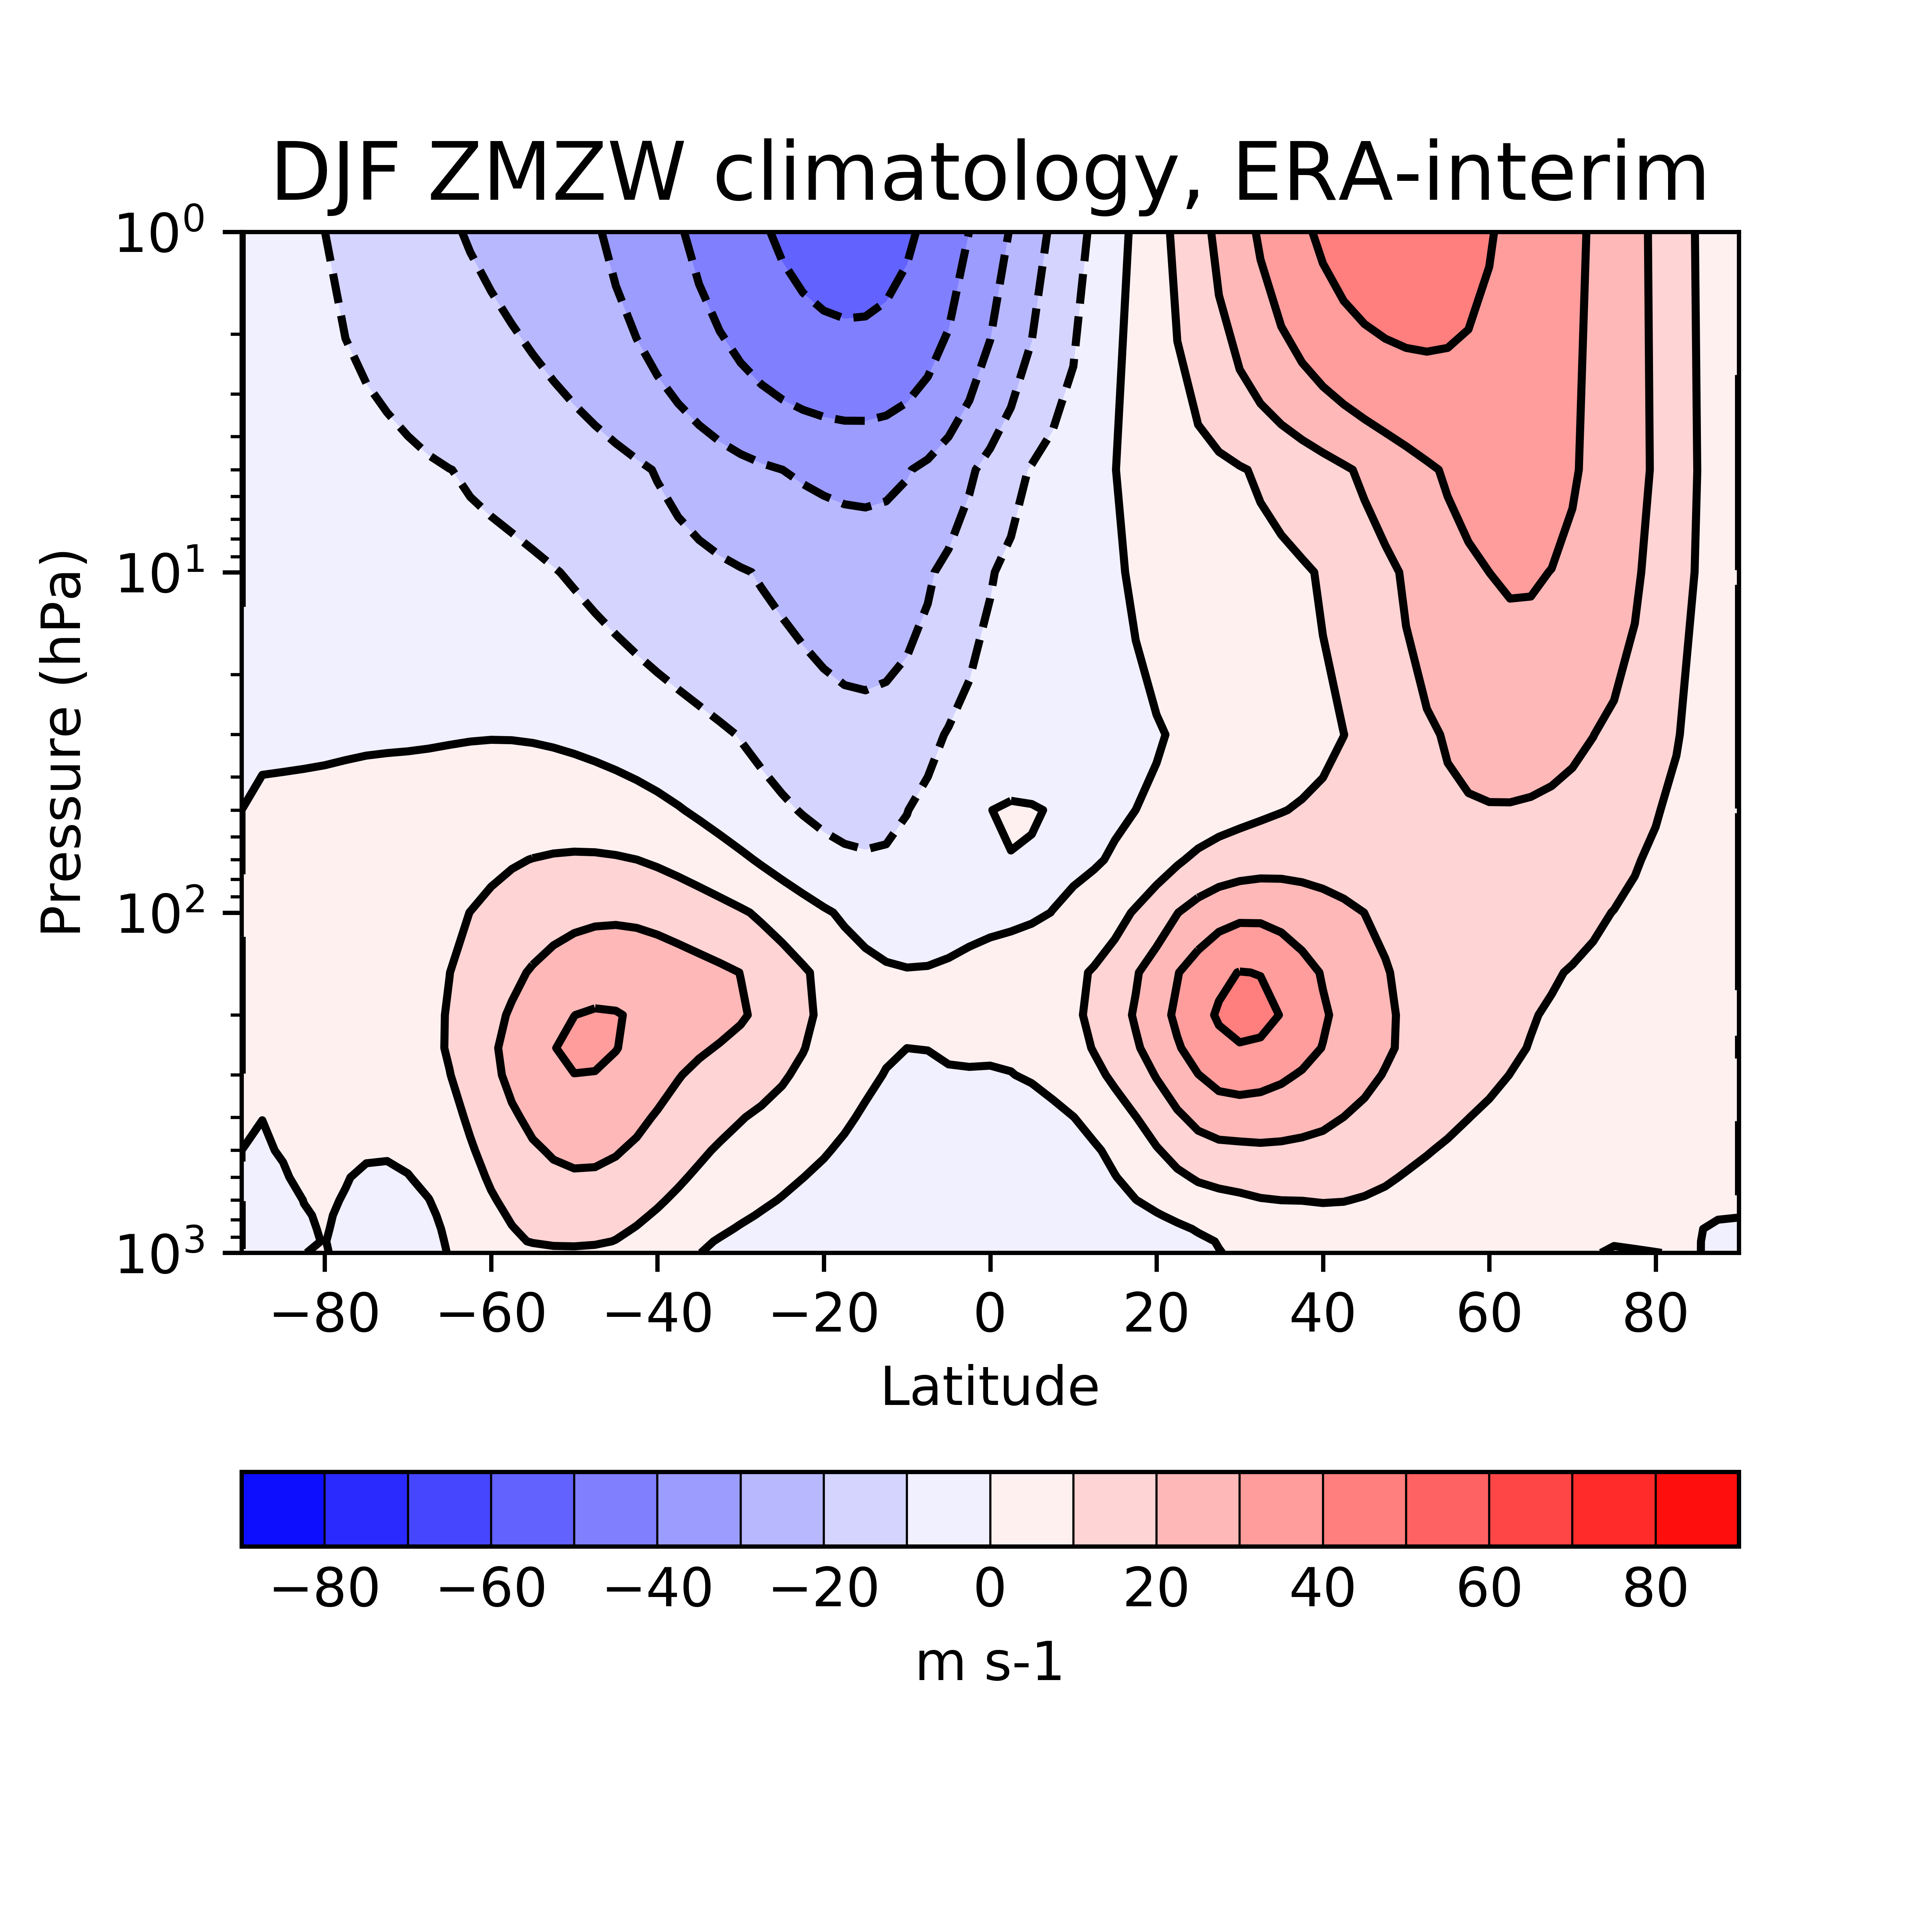
\includegraphics[width= 9cm]{Figures/Figures-background/fig1_for_transfer.png}
    \caption{DJF climatological zonal mean zonal wind from ERA-interim dataset between 1979 and 2018.}
    \label{fig:ERAclimDJF}
\centering
\end{figure}

\section{Atmospheric Waves}
\label{sec:atmos_waves}
Atmospheric wave is the term generally used for deviations from the zonal mean dynamical state and these phenomena, often referred to as Rossby waves, play a key role in the variability of the vortex. These waves are forced in the troposphere by air flowing over variations in topography (orographic waves) or through other mechanisms such as interaction with convection fronts and latent heat release (non-orographic). Perturbations originating near the surface can propagate vertically into the stratosphere altering large scale circulation features via wave drag as they transfer momentum to the background flow. 

Large scale Rossby waves are known as planetary waves and exhibit wavelengths of the order of $1000km$. The propagation of these waves can be described using the Quasi Geostrophic approximation for fluid in hydrostatic balance with low Rossby number, $R_0 = U/f_0 L$, where U and L are characteristic zonal velocity and length scales respectively. Under this framework the Quasi Geostrophic Potential Vorticity (QGPV) equation states that in the absence of friction and diabatic heating, the quasi geostrophic potential vorticity, $q$, is conserved following the geostrophic wind:

\begin{equation} \label{eq-PV_conserved}
D_g q = 0
\end{equation}

where $D_g$ is the operator 

\begin{equation}\label{eq:D_g}
D_g = \frac{\partial}{\partial t} + u_g \frac{\partial}{\partial x} + v_g\frac{\partial}{\partial y} 
\end{equation}

and $q$ can be written in terms of the stream function, $\psi$, in the QGPV framework as

\begin{equation} \label{eq:QGPV}
q = f_0 + \beta y + \nabla^2 \psi + \frac{\partial}{\partial z}\bigg(\frac{f_0^2}{N_B^2} \frac{\partial \psi}{\partial z}\bigg)
\end{equation}

where $N_B$ is the Brunt–Väisälä frequency, the frequency of vertical motion of a parcel of air in a stable atmosphere. $\psi$ is related to $u_g$ and $v_g$, the zonal and meridional components of geostrophic wind by $u_g = -\frac{\partial \psi}{\partial y}$ and $v_g = -\frac{\partial \psi}{\partial x}$. Under a further approximation of small disturbances from a uniform zonal flow, $\overline{u}$, $\psi$ is given by

\begin{equation} \label{eq:Zonal_flow_SF}
\psi = -\overline{u} y + \psi '
\end{equation}

where $\psi'$ is the contribution to the stream function from the small deviation from $\overline{u}$. This approximation allows equation \ref{eq:QGPV} to be linearised to

\begin{equation} \label{eq:Linearised_QGPV}
\bigg(\frac{\partial}{\partial t} + \overline{u} \frac{\partial}{\partial x}\bigg)\Gamma \psi' + \beta \frac{\partial \psi'}{\partial x} = 0,
\end{equation}

where $\Gamma$ is the operator

\begin{equation} \label{eq:ellipse_operator}
\Gamma = \nabla^2 \psi + \frac{\partial}{\partial z}\bigg(\frac{f_0^2}{N_B^2}\frac{\partial}{\partial z}\bigg).
\end{equation}

It can be shown that this equation has wave like solutions whose vertical propagation is only supported under the condition

\begin{equation} \label{eq:propagation_critera}
\overline{u} - c = \frac{\beta k}{k^2 + l^2 + \frac{f_0^2 m^2}{N_B^2}} < \overline{u}_c = \frac{\beta k}{k^2 + l^2}
\end{equation}

Where $\overline{u}_c$ is a critical velocity corresponding to the background flow when $m = 0$, $c$ is the phase speed and $k, l$ and $m$ are the meridional, zonal and vertical wavenumbers of the wave respectively. Also imposing that, as $m^2 > 0$, $\overline{u} - c > 0$ as well as assuming stationary waves ($c = 0$) gives the Charney-Drazin criterion for the vertical propagation of planetary waves,

\begin{equation} \label{eq:Charney-Drazin}
0 < \overline{u} < \overline{u}_c.
\end{equation}

This result implies that vertical propagation can only occur through background westerly zonal flow with a magnitude less than some critical value, $U_c$, which depends on the horizontal wavenumbers of the wave. More specifically, equation \ref{eq:propagation_critera} shows that smaller wave-numbers (larger wavelengths) favours greater propagation and is the reason the majority of wave-mean flow interactions involving the vortex occur with disturbances of wavenumbers 1-3 (referred to as wave-n disturbances). 

The Charney-Drazin criterion also leads to the definition of a critical layer of the atmosphere as the layer at which the background zonal flow no longer supports propagation of a given wave (i.e. where $\overline{u} \sim \overline{u}_c$). When a wave encounters a critical layer, much of the linear dynamical behaviour proposed in equations \ref{eq:Linearised_QGPV} breaks down as the waves' amplitude grows too large to support continued propagation and the wave dissipates, transferring momentum to the background flow through so called wave-mean flow interactions. There therefore exists a two way interaction between the background flow and wave disturbances in the atmosphere: the magnitude of $\overline{u}$ relative to $\overline{u}_c$ dictates the propagation of waves through the troposphere into the stratosphere and waves significantly influence the background wind upon dissipation at a critical layer.

Wave-mean flow momentum deposition which is key for understanding stratospheric dynamical variability can be quantified via the introduction of a variable known as the Eliassen-Palm flux. In the QG framework as above, equations for the zonal mean and eddy components of the wind vector ($u, v$) and buoyancy ($b$), the vertical acceleration of air parcels due to density variations, can be expressed as 

\begin{equation} \label{eq:QG_Ubar}
\frac{\partial \overline{u}}{\partial t} = f\overline{v} - \frac{\partial}{\partial y} \overline{u'v'} + \overline{X}, 
\end{equation}

\begin{equation} \label{eq:QG_theta}
\frac{\partial \overline{b}}{\partial t} = -N^2\overline{w} - \frac{\partial}{\partial y} \overline{v'b'} + \overline{Q}, 
\end{equation}

where the overbar denotes a zonal mean quantities and deviations from this (eddy quantities) are denoted by primes. $\overline{X}$ and $\overline{Y}$ represent the dissipative forces on the flow (in this case friction and diabatic heating). Buoyancy is used in these equations as a close analogous of temperature. $b = g\frac{T - T_r}{T_r}$ where $T_r$ is a reference temperature normally defined by height. $b$ is related to the concept of reduced gravity which is important when considering vertical fluid motion. 

In order to decouple these equations, we introduce the mean residual circulation, the difference between zonal mean flow and contributions from eddy-mean flow interactions. These are known as the Transformed Eulerian Mean (TEM) meridional and vertical velocities \citep{Andrews1976} (denoted by $^*$) and can be expressed as 

\begin{equation} \label{eq:V*}
\overline{v^*} = \overline{v} - \frac{1}{\rho_0}\frac{\partial}{\partial z} \bigg(\rho_0 \frac{\overline{v'\theta'}}{\frac{\partial{\overline{\theta}}}{\partial{z}}}\bigg)
\end{equation}\break
\begin{equation} \label{eq:W*}
\overline{w^*} = \overline{w} + \frac{\partial}{\partial y} \bigg( \frac{\overline{v'b'}}{\frac{\partial{\overline{\theta}}}{\partial{z}}}\bigg).
\end{equation}


Under these transformations the decoupled equations can be written as

\begin{equation} \label{eq:decoupled_U}
\frac{\partial \overline{u}}{\partial t} - f_0 \overline{v*} = \frac{1}{\rho_0} (\nabla \cdot F) + \overline{X}
\end{equation}

and

\begin{equation} \label{eq:decoupled_b}
\frac{\partial \overline{b}}{\partial t} + N^2 \overline{w*} = \overline{Q},
\end{equation}

where

\begin{equation} \label{eq:EP_flux}
F = -\rho_0 \overline{u'v'}\textbf{j} + f\rho_0\frac{\overline{v'\theta'}}{\frac{\partial{\overline{\theta}}}{\partial{z}}} \textbf{k}
\end{equation}

is the Eliassen-Palm flux which can be thought of as the flux of wave activity in the meridional and vertical directions (\textbf{j} and \textbf{k} represent unit vectors in the $y$ and $z$ directions) \citep{Andrews1976}. These equations indicate that EP flux divergence ($\nabla \cdot F > 0$) signifies momentum dissipation accelerating the ZMZW ($\overbar{u}$). Conversely, flux convergence ($\nabla \cdot F < 0$) indicates deceleration in ZMZW due to wave dissipation.

\subsection{Other Atmospheric Waves} \label{sec:other_waves}
In addition to planetary scale Rossby waves outlined in previous sections, other types of wave play a vital role in stratospheric variability. Gravity waves arise due to buoyancy variations and, similarly to planetary waves, can be forced through airflow over variations in topography (orographic) or convection fronts (non orographic). These waves exhibit length scales significantly shorter than planetary waves ($\sim xxxm$) and are often not explicitly represented in general circulation models (GCMs) due to horizontal resolution issues. Instead their effects are parameterised and appear in the dissipative force term ($\overline{X}$) in in equation \ref{eq:QG_Ubar}

Kelvin waves occur when air is trapped between regions in which Coriolis force terms act in opposite directions. In these regions, geostrophic balance does not apply and the waves exhibit a westerly phase velocity. Dissipation of these waves contributes westerly momentum to the background flow. Finally, Rossby-gravity waves exhibit different behaviour for small and large length scales (or horizontal wave number, $k$). for small $k$ (large length scale), they reduce to Rossby wavelike disturbances, similar to planetary scale Rossby waves outlined in the previous section in which variations in Coriolis parameter with latitude act as the restoring force. For large $k$ (shorter length scales), they behave as gravity waves (those for which the restoring force is gravity). Rossby-gravity waves typically have easterly phase velocity and contribute easterly momentum to background flow upon dissipation \citep{Andrews1976}.

\section{Sudden Stratospheric Warmings}
While the vortex generally exhibits strong, westerly flow over the boreal winter, it can be significantly disrupted on sub-seasonal timescales
(see individual season winds on figure \ref{fig:ERAclimDJF}b). This reversal occurs due to the dissipation of planetary waves on the vortex depositiong easterly momentum on the backgroud flow. If this deposition is large enough such that the westerly flow reverses an event known as a sudden stratospheric warming (SSW) occurs. Such events are named as they are often associated with significant and rapid increases in middle atmosphere polar cap temperature ($\sim~50K$ over a few days) and they were first observed in radiosonde data in Scherberg et al. 1952 (ref xxxx). In observation based datasets SSWs occur at an average rate of xxxx events per decade and represent one of the largest modes of interannual variability in the NH stratosphere.

Matsuno 1971 was the first work to introduce a dynamical model linking the action of planetary waves and the occurence of SSWs. The framework developed by this work is still largely accepted today and describes the mechanisms involved in the life cycle of an SSW as follows. First, a burst of planetary wave activity is generated in the troposphere through a combination of airflow of topography and convection fronts. Waves subsequently propagate into the stratosphere in accordance with the Charney-Drazin criterion. When these waves encounter a critical layer (normally one which exhibits stronger westerlies than $U_c$ as the undisturbed vortex is strong) these waves break and dissipate easterly momentum to the background zonal flow. As a result, the westerly vortex decelerates and, if the planetary wave activity is strong enough, even reverses. As a result, new critical layers are formed (where $\overline{u} = 0$) at a level below that of the original reversal. Subsequent waves now dissipate and can act to reverse the background flow at this lower critical layer. This process repeats and the critical layers can descend into the lower stratosphere. Once the critical layer lies near the tropopause, planetary waves are effectively prevented from entering the stratosphere stopping further deceleration of the vortex. With wave driving of the vortex prevented, radiative cooling of the stratosphere subsequently bring polar cap temperatures back down and the strong westerly flow of the vortex recovers. 

This framework provides a mechanism by which SSWs occur through planetary waves influencing the zonal mean flow. However, further studies show that as well as zonal mean disturbance, the geometry of the vortex is altered significantly during these event. The vortex can either be shifted from its stable centroid to a lower latitude or split into two daughter vortices (each of which exhibits a core of high PV air). It's further shown in xxxx et al. that the type of deformation occurring depends on the wave number of the dominant planetary waves involved with wave-1 disturbances more associated with displacement events and wave-2 with split events. Figure xxxx demonstrates the three vortex configurations: stable (strong vortex), displaced and split.


\section{The Equatorial Stratosphere}\label{sec:equatorial_strat}
Another region which exhibits key modes of stratospheric dynamical variability is to the equatorial region. The most notable of these modes are the quasi-biennial oscillation the zonal flow which varies with a frequency of approximately 28-29 months between the 100\,hPa and 10\,hPa levels and the semiannual oscillation of zonal wind which cycles more regularly with a frequency of 6 months around the 1\,hPa level (figure \ref{fig:QBO_SAO_ERA}) \citep{Baldwin2001}.

\begin{figure}[h!]
\centering
    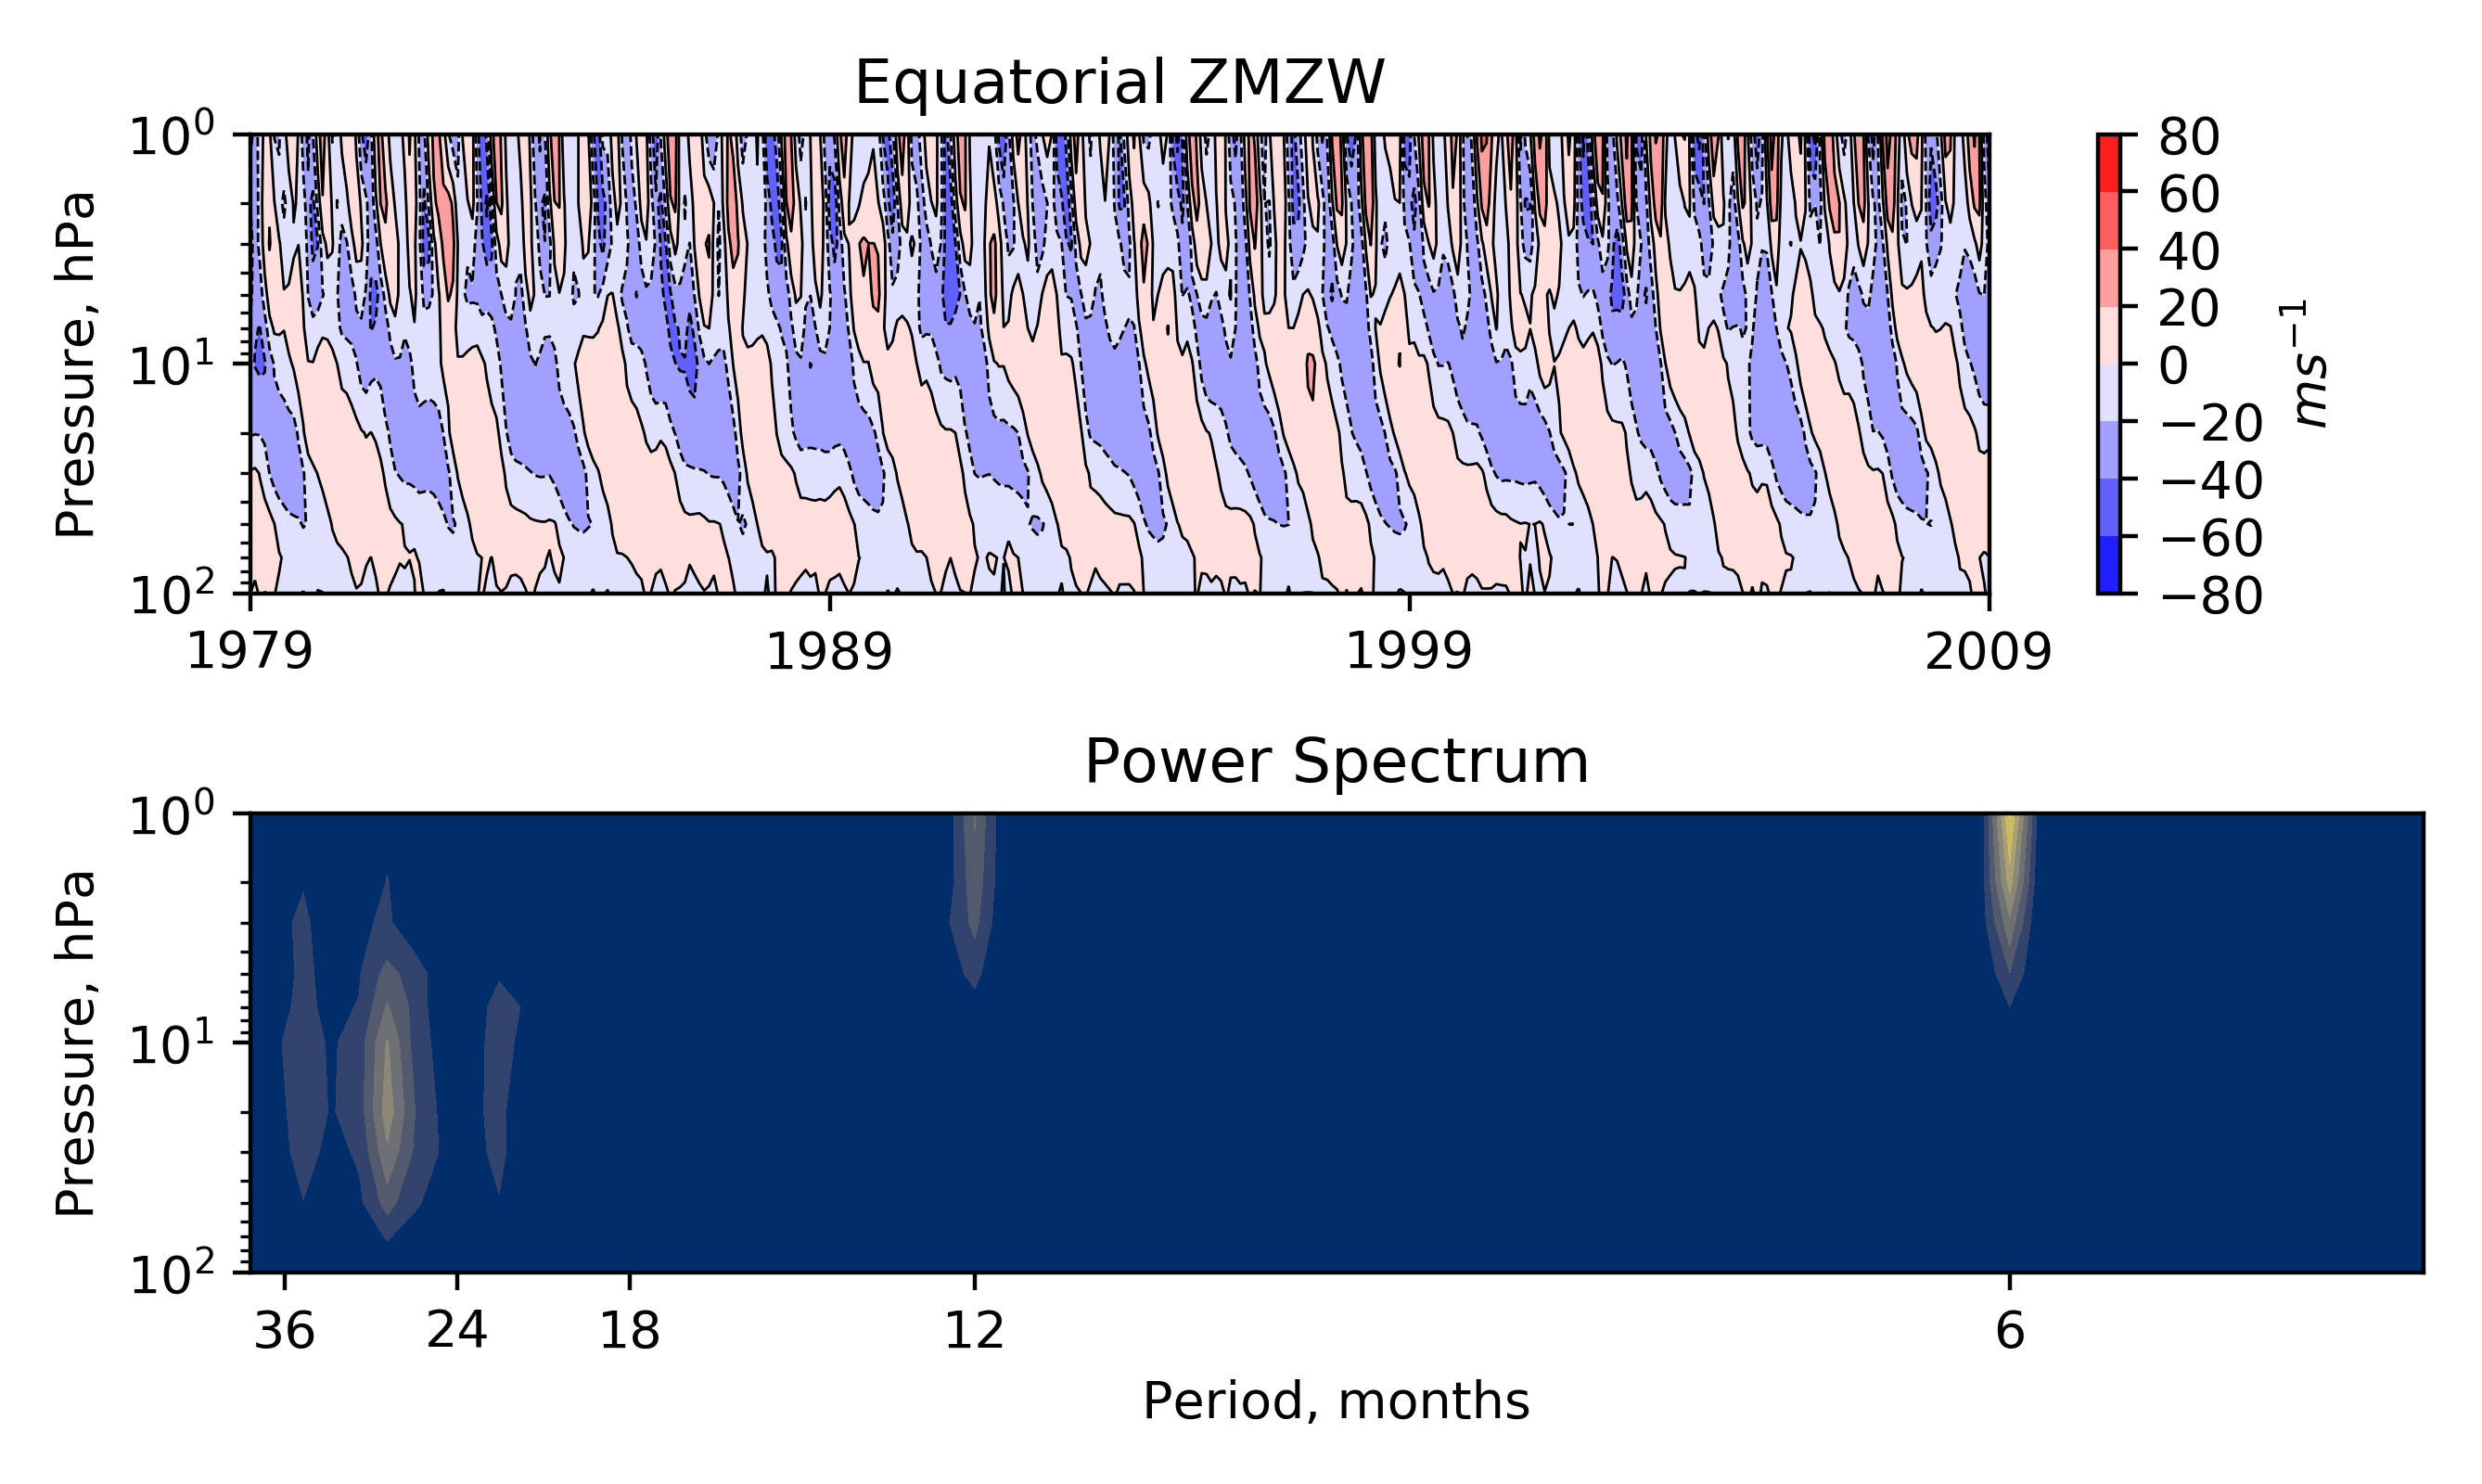
\includegraphics[width=0.88\textwidth]{Figures/Figures-background/QBO_SAO_ERA.png}
    \caption{Equatorial ZMZW (top) and associated power spectrum (bottom) for the ERA-Interim dataset between 1979 and 2009.}
    \label{fig:QBO_SAO_ERA}
\centering
\end{figure}
\FloatBarrier

The QBO was first fully classified as a phenomenon using balloon based observations in \cite{Ebdon1960} and \cite{Reed1964}. These studies found a set of descending shears of easterly and westerly ZMZW above the equator between approximately the 10hPa and 100hPa pressure levels. These seminal studies made use of a short observational record (approximately 5 years) and later works with more comprehensive observation based datasets were able to establish the key features of the oscillation \citep{Baldwin2001,Pascoe2005}. These include an approximate period of 28.1 months (although a range of 22-40 months is also recorded)  with an asymmetry in the rate of descent of the westerly and easterly phases - slower descending easterly winds are caused by increased equatorial upwelling associated with this phase \citep{Pascoe2005}. The oscillation is generally zonally symmetric \citep{BELMONT1968} and has a latitudinal extent of approximately $12^{\circ}$ half width at half maximum \citep{Baldwin2001}.

The primary cause of the oscillation is the interaction of waves outlined in section \ref{waves} with the background zonal flow. To analyse the action of these waves, consider a pair of equatorial waves with phase speeds of $+c $ and $-c$ respectively (figure \ref{fig:QBO_wave_schematic})  \citep{Plumb1984}). These waves will propagate or dissipate according to the difference between their phase speed and the background flow, $\overbar{u}$. If $\overbar{u}$ approaches $+c$ or $-c$ at a given height, the respective wave will deposit momentum of the same sign as its phase speed onto the background flow. This means that, for a background wind profile like that shown in \ref{fig:QBO_wave_schematic}a, westerly momentum is deposited at the bottom of a zone of westerly low altitude background wind, while easterly phase speed waves pass through and are deposited above on easterly flow. Viscous body acceleration counteract these wave accelerations leading to profiles in figure \ref{fig:QBO_wave_schematic}b where westerly waves pass through the flow and easterlies deposit momentum. Finally westerly waves begin to accelerate flow from high levels descending to finally force the background profile to figure \ref{fig:QBO_wave_schematic}d which is the inverse of schematic a. The asymmetry in descent speed between phases of the QBO is accounted for by the induced meridional circulation associated with each phase. An easterly QBO in the lower stratosphere induces a poleward meridional circulation at the same level \citep{plumb82,Baldwin2001} as well as an acceleration in upwelling over the equator, this slows the descent of the QBO easterlies \citep{Reed1964}. The converse is true for a westerly phase in the lower stratosphere. 

\begin{figure}[h!]
\centering
    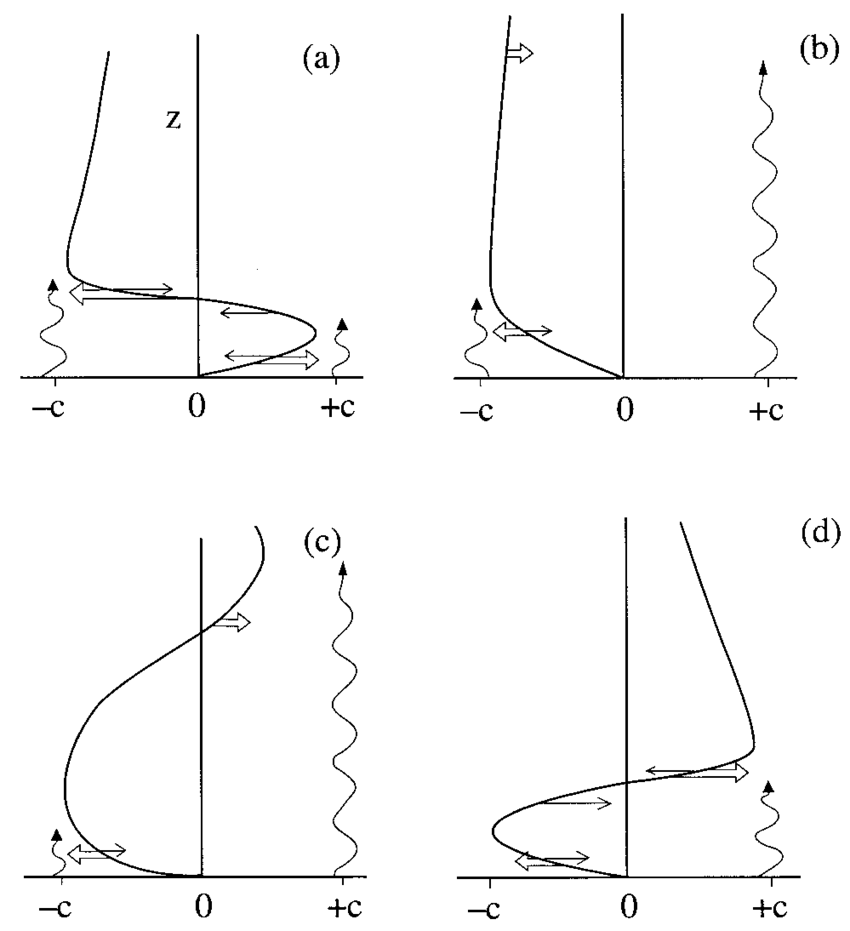
\includegraphics[width=0.5\textwidth]{Figures/Figures-background/Schematic_of_QBO_waves.png}
    \caption{Schematic of equatorial wave-mean flow interactions for 2 example wave disturbances (phase speeds $^+_- c$) from \cite{Plumb1984}. Solid continuous lines show the background flow of the QBO in developing phases, wavy arrows indicate propagation of the 2 waves, double arrows show momentum deposition on the mean flow from wave breaking, single arrows indicate viscous-driven acceleration.}
    \label{fig:QBO_wave_schematic}
\centering
\end{figure}
\section{Stratosphere-Troposphere Coupling and Surface Variability}
\section{Stratosphere-Ocean Interactions}


